% -*- mode: latex; mode: flyspell; ispell-local-dictionary: "en_US"; coding: utf-8 -*-

\documentclass{standalone}

\usepackage[utf8]{inputenc}
\usepackage[english]{babel}

\usepackage{amsmath,amsfonts,amssymb}

\usepackage{tikz,pgfplots}
\usetikzlibrary{plotmarks}
\pgfplotsset{compat=newest}

\usepgfplotslibrary{groupplots}
\pgfplotsset{every axis/.style={scale only axis}}

\pgfplotsset{
  major grid style={dashed},
  minor grid style={thin,dotted},
  ymajorgrids,
  yminorgrids,
  every axis/.append style={
    line width=0.7pt,
    tick style={
      line cap=round,
      thin,
      major tick length=4pt,
      minor tick length=2pt,
    },
  },
  legend cell align=left,
  legend style={
    line width=0.7pt,
    /tikz/every even column/.append style={column sep=3mm,black},
    /tikz/every odd column/.append style={black},
  },
  % move title closer
  legend style={font=\small},
  title style={yshift=-2pt},
  % less space on left and right
  enlarge x limits=0.04,
  every tick label/.append style={font=\footnotesize},
  every axis label/.append style={font=\small},
  every axis y label/.append style={yshift=-1ex},
  /pgf/number format/1000 sep={},
  axis lines*=left,
  xlabel near ticks,
  ylabel near ticks,
  axis lines*=left,
  label style={font=\footnotesize},       
  tick label style={font=\footnotesize},
  plotParallel/.style={
    width=38mm,
    height=20mm,
  },
  parLZ/.style={
    mark=x,
    mark options={solid},
    my-deep-orange,
    dotted,
  },
  parWoRS/.style={
    mark=pentagon,
    mark options={solid},
    my-light-blue,
    dotted,
  },
  parRS/.style={
    mark=+,
    mark options={solid},
    my-deep-purple,
    dotted,
  },
}


\usepackage{xcolor}
\definecolor{my-dark-red}{RGB}{183, 28, 28}
\definecolor{my-red}{RGB}{244,67,54}
\definecolor{my-pink}{RGB}{233,30,99}
\definecolor{my-purple}{RGB}{156,39,176}
\definecolor{my-deep-purple}{RGB}{103,58,183}
\definecolor{my-indigo}{RGB}{63,81,181}
\definecolor{my-blue}{RGB}{33,150,243}
\definecolor{my-light-blue}{RGB}{3,169,244}
\definecolor{my-cyan}{RGB}{0,188,212}
\definecolor{my-teal}{RGB}{0,150,136}
\definecolor{my-green}{RGB}{76,175,80}
\definecolor{my-light-green}{RGB}{139,195,74}
\definecolor{my-lime}{RGB}{205,220,57}
\definecolor{my-yellow}{RGB}{255,235,59}
\definecolor{my-amber}{RGB}{255,193,7}
\definecolor{my-orange}{RGB}{255,152,0}
\definecolor{my-deep-orange}{RGB}{255,87,34}
\definecolor{my-brown}{RGB}{121,85,72}
\definecolor{my-grey}{RGB}{158,158,158}
\definecolor{my-blue-grey}{RGB}{96,125,139}
\definecolor{my-lipics-grey}{rgb}{0.6,0.6,0.61}


\colorlet{fp1Color}{my-blue}
\colorlet{fpzColor}{my-blue}
\colorlet{lpf1Color}{my-green}
\colorlet{lpfzColor}{my-green}
\colorlet{lpf1dpColor}{my-deep-orange}
\colorlet{lpfzdpColor}{my-deep-orange}
\colorlet{belazzouguiColor}{my-dark-red}

\begin{document}

% IMPORT-DATA our_stats ./data/repetitive_our.txt
% IMPORT-DATA belazzougui_stats ./data/repetitive_belazzougui.txt
% IMPORT-DATA algorithm_meta_data ./data/algorithm_names.txt
% IMPORT-DATA parallel_stats ./data/repetitive_our_parallel.txt


\begin{tabular}{rrr}
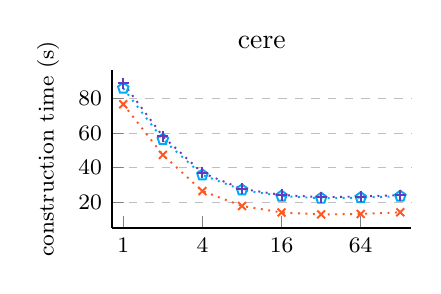
\begin{tikzpicture}
\begin{axis}[
  title={cere},
  ylabel={construction time (s)},
  xmode=log,
  log basis x={2},
  %ymode=log,
  log ticks with fixed point,
  plotParallel,
  legend to name={leg:construction_parallel}
  ]

%% MULTIPLOT(algorithm|ptitle|attr)
%% SELECT threads AS x, AVG(lz_and_z_time/1000.0) AS y, "par \LPF" as ptitle, "parLZ" AS attr, MULTIPLOT
%% FROM parallel_stats
%% JOIN algorithm_meta_data ON algorithm = algorithm_name
%% WHERE input LIKE '%cere%' AND tau=4 AND max_leaf_size=16
%% GROUP BY MULTIPLOT,x ORDER BY sorting_order
\addplot[parLZ] coordinates { (1,76.6573) (2,47.438) (4,26.5687) (8,17.9623) (16,14.222) (32,13.0747) (64,13.371) (128,14.303) };
\addlegendentry{par \LPF};
  
%% MULTIPLOT(algorithm|ptitle|attr)
%% SELECT threads AS x, AVG(construction_time_ms/1000.0) AS y, "par BT w/o RS" as ptitle, "parWoRS" AS attr, MULTIPLOT
%% FROM parallel_stats
%% JOIN algorithm_meta_data ON algorithm = algorithm_name
%% WHERE input LIKE '%cere%' AND tau=4 AND max_leaf_size=16
%% GROUP BY MULTIPLOT,x ORDER BY sorting_order
\addplot[parWoRS] coordinates { (1,85.87) (2,56.3573) (4,35.827) (8,27.2077) (16,23.6413) (32,22.39) (64,22.755) (128,23.5723) };
\addlegendentry{par BT w/o RS};

  
%% MULTIPLOT(algorithm|ptitle)
%% SELECT threads AS x, AVG(construction_time_with_rs_ms/1000.0) AS y, "par BT with RS" as ptitle, "parRS" AS attr,MULTIPLOT
%% FROM parallel_stats
%% JOIN algorithm_meta_data ON algorithm = algorithm_name
%% WHERE input LIKE '%cere%' AND tau=4 AND max_leaf_size=16
%% GROUP BY MULTIPLOT,x ORDER BY sorting_order
\addplot[parRS] coordinates { (1,88.767) (2,58.1467) (4,37.03) (8,27.8357) (16,24.277) (32,23.0323) (64,23.393) (128,24.206) };
\addlegendentry{par BT with RS};

\end{axis}
\end{tikzpicture}
  &
    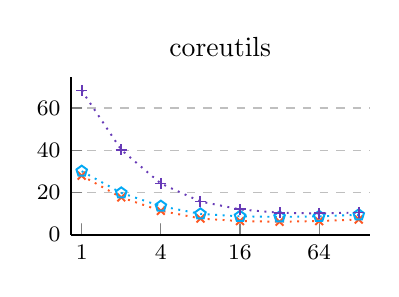
\begin{tikzpicture}
\begin{axis}[
  title={coreutils},
  xmode=log,
  log basis x={2},
    log ticks with fixed point,
  %%ymode=log,
  log basis y={2},
  plotParallel,
  %ymajorticks=false,
]
%% MULTIPLOT(algorithm|ptitle|attr)
%% SELECT threads AS x, AVG(lz_and_z_time/1000.0) AS y, "par \LPF" as ptitle, "parLZ" AS attr, MULTIPLOT
%% FROM parallel_stats
%% JOIN algorithm_meta_data ON algorithm = algorithm_name
%% WHERE input LIKE '%coreutils%' AND tau=4 AND max_leaf_size=16
%% GROUP BY MULTIPLOT,x ORDER BY sorting_order
\addplot[parLZ] coordinates { (1,27.903) (2,17.594) (4,11.2443) (8,7.57967) (16,6.34767) (32,6.05433) (64,6.37067) (128,7.08467) };
\addlegendentry{par \LPF};
  
%% MULTIPLOT(algorithm|ptitle|attr)
%% SELECT threads AS x, AVG(construction_time_ms/1000.0) AS y, "par BT w/o RS" as ptitle, "parWoRS" AS attr, MULTIPLOT
%% FROM parallel_stats
%% JOIN algorithm_meta_data ON algorithm = algorithm_name
%% WHERE input LIKE '%coreutils%' AND tau=4 AND max_leaf_size=16
%% GROUP BY MULTIPLOT,x ORDER BY sorting_order
\addplot[parWoRS] coordinates { (1,30.0277) (2,19.7173) (4,13.4343) (8,9.76067) (16,8.61267) (32,8.32833) (64,8.59933) (128,9.325) };
\addlegendentry{par BT w/o RS};

  
%% MULTIPLOT(algorithm|ptitle|attr)
%% SELECT threads AS x, AVG(construction_time_with_rs_ms/1000.0) AS y, "par BT with RS" as ptitle, "parRS" AS attr, MULTIPLOT
%% FROM parallel_stats
%% JOIN algorithm_meta_data ON algorithm = algorithm_name
%% WHERE input LIKE '%coreutils%' AND tau=4 AND max_leaf_size=16
%% GROUP BY MULTIPLOT,x ORDER BY sorting_order
\addplot[parRS] coordinates { (1,68.293) (2,40.1207) (4,24.1747) (8,15.638) (16,11.891) (32,10.2817) (64,9.98433) (128,10.4233) };
\addlegendentry{par BT with RS};
\legend{};

\end{axis}
\end{tikzpicture}
  &
    \raisebox{1cm}{\ref*{leg:construction_parallel}}
    \hspace{.5cm}
  \\
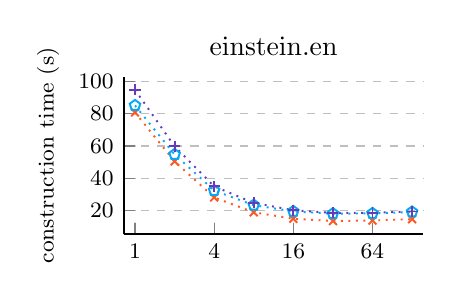
\begin{tikzpicture}
\begin{axis}[
  title={einstein.en},
  ylabel={construction time (s)},
  xmode=log,
  log basis x={2},
  %ymode=log,
  log ticks with fixed point,
  plotParallel,
]
%% MULTIPLOT(algorithm|ptitle|attr)
%% SELECT threads AS x, AVG(lz_and_z_time/1000.0) AS y, "par \LPF" as ptitle, "parLZ" AS attr, MULTIPLOT
%% FROM parallel_stats
%% JOIN algorithm_meta_data ON algorithm = algorithm_name
%% WHERE input LIKE '%einstein.en.txt%' AND tau=4 AND max_leaf_size=16
%% GROUP BY MULTIPLOT,x ORDER BY sorting_order
\addplot[parLZ] coordinates { (1,80.9077) (2,50.4703) (4,28.0517) (8,18.81) (16,14.8297) (32,13.41) (64,13.756) (128,14.568) };
\addlegendentry{par \LPF};
  
%% MULTIPLOT(algorithm|ptitle|attr)
%% SELECT threads AS x, AVG(construction_time_ms/1000.0) AS y, "par BT w/o RS" as ptitle, "parWoRS" AS attr, MULTIPLOT
%% FROM parallel_stats
%% JOIN algorithm_meta_data ON algorithm = algorithm_name
%% WHERE input LIKE '%einstein.en.txt%' AND tau=4 AND max_leaf_size=16
%% GROUP BY MULTIPLOT,x ORDER BY sorting_order
\addplot[parWoRS] coordinates { (1,85.2327) (2,54.7817) (4,32.3463) (8,23.2463) (16,19.365) (32,17.979) (64,18.1497) (128,19.042) };
\addlegendentry{par BT w/o RS};

  
%% MULTIPLOT(algorithm|ptitle|attr)
%% SELECT threads AS x, AVG(construction_time_with_rs_ms/1000.0) AS y, "par BT with RS" as ptitle, "parRS" AS attr, MULTIPLOT
%% FROM parallel_stats
%% JOIN algorithm_meta_data ON algorithm = algorithm_name
%% WHERE input LIKE '%einstein.en.txt%' AND tau=4 AND max_leaf_size=16
%% GROUP BY MULTIPLOT,x ORDER BY sorting_order
\addplot[parRS] coordinates { (1,94.967) (2,59.8343) (4,34.9427) (8,24.666) (16,20.1333) (32,18.4367) (64,18.477) (128,19.3177) };
\addlegendentry{par BT with RS};

\legend{};

\end{axis}
\end{tikzpicture}
  &
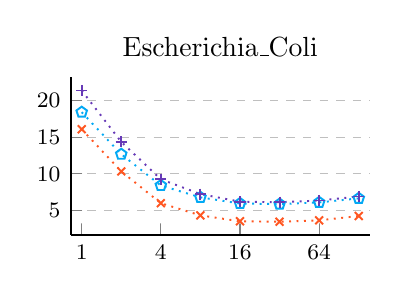
\begin{tikzpicture}
\begin{axis}[
  title={Escherichia\_Coli},
  xmode=log,
  log basis x={2},
  %ymode=log,
  log ticks with fixed point,
  plotParallel,
]
%% MULTIPLOT(algorithm|ptitle|attr)
%% SELECT threads AS x, AVG(lz_and_z_time/1000.0) AS y, "par \LPF" as ptitle, "parLZ" AS attr, MULTIPLOT
%% FROM parallel_stats
%% JOIN algorithm_meta_data ON algorithm = algorithm_name
%% WHERE input LIKE '%Escherichia_Coli%' AND tau=4 AND max_leaf_size=16
%% GROUP BY MULTIPLOT,x ORDER BY sorting_order
\addplot[parLZ] coordinates { (1,16.068) (2,10.3373) (4,6.01567) (8,4.362) (16,3.55533) (32,3.49833) (64,3.69) (128,4.27567) };
\addlegendentry{par \LPF};
  
%% MULTIPLOT(algorithm|ptitle|attr)
%% SELECT threads AS x, AVG(construction_time_ms/1000.0) AS y, "par BT w/o RS" as ptitle, "parWoRS" AS attr, MULTIPLOT
%% FROM parallel_stats
%% JOIN algorithm_meta_data ON algorithm = algorithm_name
%% WHERE input LIKE '%Escherichia_Coli%' AND tau=4 AND max_leaf_size=16
%% GROUP BY MULTIPLOT,x ORDER BY sorting_order
\addplot[parWoRS] coordinates { (1,18.3817) (2,12.6657) (4,8.418) (8,6.80833) (16,5.97367) (32,5.89667) (64,6.126) (128,6.67033) };
\addlegendentry{par BT w/o RS};

  
%% MULTIPLOT(algorithm|ptitle|attr)
%% SELECT threads AS x, AVG(construction_time_with_rs_ms/1000.0) AS y, "par BT with RS" as ptitle, "parRS" AS attr, MULTIPLOT
%% FROM parallel_stats
%% JOIN algorithm_meta_data ON algorithm = algorithm_name
%% WHERE input LIKE '%Escherichia_Coli%' AND tau=4 AND max_leaf_size=16
%% GROUP BY MULTIPLOT,x ORDER BY sorting_order
\addplot[parRS] coordinates { (1,21.329) (2,14.345) (4,9.27233) (8,7.25433) (16,6.22467) (32,6.146) (64,6.37967) (128,6.926) };
\addlegendentry{par BT with RS};

\legend{};

\end{axis}
\end{tikzpicture}
  &
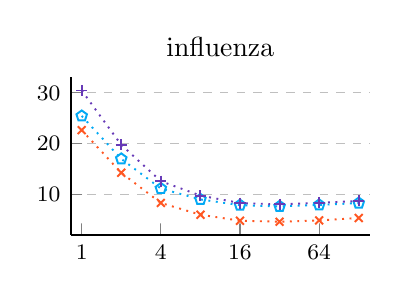
\begin{tikzpicture}
\begin{axis}[
  title={influenza},
  xmode=log,
  log basis x={2},
  %ymode=log,
  log ticks with fixed point,
  plotParallel,
]
%% MULTIPLOT(algorithm|ptitle|attr)
%% SELECT threads AS x, AVG(lz_and_z_time/1000.0) AS y, "par \LPF" as ptitle, "parLZ" AS attr, MULTIPLOT
%% FROM parallel_stats
%% JOIN algorithm_meta_data ON algorithm = algorithm_name
%% WHERE input LIKE '%influenza%' AND tau=4 AND max_leaf_size=16
%% GROUP BY MULTIPLOT,x ORDER BY sorting_order
\addplot[parLZ] coordinates { (1,22.6603) (2,14.242) (4,8.299) (8,5.97267) (16,4.79933) (32,4.59467) (64,4.85067) (128,5.34133) };
\addlegendentry{par \LPF};
  
%% MULTIPLOT(algorithm|ptitle|attr)
%% SELECT threads AS x, AVG(construction_time_ms/1000.0) AS y, "par BT w/o RS" as ptitle, "parWoRS" AS attr, MULTIPLOT
%% FROM parallel_stats
%% JOIN algorithm_meta_data ON algorithm = algorithm_name
%% WHERE input LIKE '%influenza%' AND tau=4 AND max_leaf_size=16
%% GROUP BY MULTIPLOT,x ORDER BY sorting_order
\addplot[parWoRS] coordinates { (1,25.4513) (2,16.9873) (4,11.143) (8,8.99333) (16,7.862) (32,7.61467) (64,7.911) (128,8.27533) };
\addlegendentry{par BT w/o RS};

  
%% MULTIPLOT(algorithm|ptitle|attr)
%% SELECT threads AS x, AVG(construction_time_with_rs_ms/1000.0) AS y, "par BT with RS" as ptitle, "parRS" AS attr, MULTIPLOT
%% FROM parallel_stats
%% JOIN algorithm_meta_data ON algorithm = algorithm_name
%% WHERE input LIKE '%influenza%' AND tau=4 AND max_leaf_size=16
%% GROUP BY MULTIPLOT,x ORDER BY sorting_order
\addplot[parRS] coordinates { (1,30.4763) (2,19.758) (4,12.587) (8,9.756) (16,8.27667) (32,8.02933) (64,8.32833) (128,8.692) };
\addlegendentry{par BT with RS};

\legend{};

\end{axis}
\end{tikzpicture}
  \\
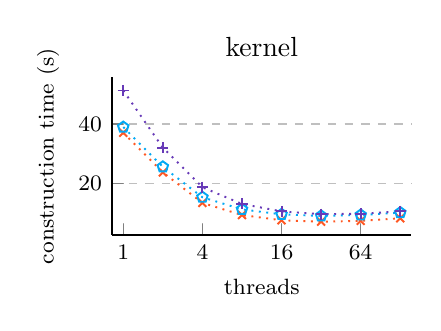
\begin{tikzpicture}
\begin{axis}[
  title={kernel},
  xlabel={threads},
  ylabel={construction time (s)},
  xmode=log,
  log basis x={2},
  %ymode=log,
  log ticks with fixed point,
  plotParallel,
]
%% MULTIPLOT(algorithm|ptitle|attr)
%% SELECT threads AS x, AVG(lz_and_z_time/1000.0) AS y, "par \LPF" as ptitle, "parLZ" AS attr, MULTIPLOT
%% FROM parallel_stats
%% JOIN algorithm_meta_data ON algorithm = algorithm_name
%% WHERE input LIKE '%kernel%' AND tau=4 AND max_leaf_size=16
%% GROUP BY MULTIPLOT,x ORDER BY sorting_order
\addplot[parLZ] coordinates { (1,37.082) (2,23.8363) (4,13.6187) (8,9.56067) (16,7.82533) (32,7.331) (64,7.61267) (128,8.47367) };
\addlegendentry{par \LPF};
  
%% MULTIPLOT(algorithm|ptitle|attr)
%% SELECT threads AS x, AVG(construction_time_ms/1000.0) AS y, "par BT w/o RS" as ptitle, "parWoRS" AS attr, MULTIPLOT
%% FROM parallel_stats
%% JOIN algorithm_meta_data ON algorithm = algorithm_name
%% WHERE input LIKE '%kernel%' AND tau=4 AND max_leaf_size=16
%% GROUP BY MULTIPLOT,x ORDER BY sorting_order
\addplot[parWoRS] coordinates { (1,38.959) (2,25.6757) (4,15.5063) (8,11.451) (16,9.78233) (32,9.27533) (64,9.58) (128,10.3703) };
\addlegendentry{par BT w/o RS};

  
%% MULTIPLOT(algorithm|ptitle|attr)
%% SELECT threads AS x, AVG(construction_time_with_rs_ms/1000.0) AS y, "par BT with RS" as ptitle, "parRS" AS attr, MULTIPLOT
%% FROM parallel_stats
%% JOIN algorithm_meta_data ON algorithm = algorithm_name
%% WHERE input LIKE '%kernel%' AND tau=4 AND max_leaf_size=16
%% GROUP BY MULTIPLOT,x ORDER BY sorting_order
\addplot[parRS] coordinates { (1,51.193) (2,32.0987) (4,18.85) (8,13.268) (16,10.7913) (32,9.85733) (64,10.0233) (128,10.763) };
\addlegendentry{par BT with RS};

\legend{};

\end{axis}
\end{tikzpicture}
  &
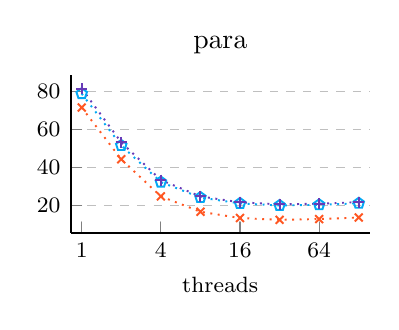
\begin{tikzpicture}
\begin{axis}[
  title={para},
  xlabel={threads},
  xmode=log,
  log basis x={2},
  log ticks with fixed point,
  %ymode=log,
  plotParallel,
]
%% MULTIPLOT(algorithm|ptitle|attr)
%% SELECT threads AS x, AVG(lz_and_z_time/1000.0) AS y, "par \LPF" as ptitle, "parLZ" AS attr, MULTIPLOT
%% FROM parallel_stats
%% JOIN algorithm_meta_data ON algorithm = algorithm_name
%% WHERE input LIKE '%para%' AND tau=4 AND max_leaf_size=16
%% GROUP BY MULTIPLOT,x ORDER BY sorting_order
\addplot[parLZ] coordinates { (1,71.628) (2,44.3623) (4,24.826) (8,16.7363) (16,13.423) (32,12.4807) (64,12.882) (128,13.706) };
\addlegendentry{par \LPF};
  
%% MULTIPLOT(algorithm|ptitle|attr)
%% SELECT threads AS x, AVG(construction_time_ms/1000.0) AS y, "par BT w/o RS" as ptitle, "parWoRS" AS attr, MULTIPLOT
%% FROM parallel_stats
%% JOIN algorithm_meta_data ON algorithm = algorithm_name
%% WHERE input LIKE '%para%' AND tau=4 AND max_leaf_size=16
%% GROUP BY MULTIPLOT,x ORDER BY sorting_order
\addplot[parWoRS] coordinates { (1,78.933) (2,51.6333) (4,32.369) (8,24.2353) (16,21.1157) (32,20.047) (64,20.4017) (128,21.2007) };
\addlegendentry{par BT w/o RS};

  
%% MULTIPLOT(algorithm|ptitle|attr)
%% SELECT threads AS x, AVG(construction_time_with_rs_ms/1000.0) AS y, "par BT with RS" as ptitle, "parRS" AS attr, MULTIPLOT
%% FROM parallel_stats
%% JOIN algorithm_meta_data ON algorithm = algorithm_name
%% WHERE input LIKE '%para%' AND tau=4 AND max_leaf_size=16
%% GROUP BY MULTIPLOT,x ORDER BY sorting_order
\addplot[parRS] coordinates { (1,81.6257) (2,53.306) (4,33.4437) (8,24.816) (16,21.709) (32,20.6373) (64,20.9967) (128,21.79) };
\addlegendentry{par BT with RS};

\legend{};

\end{axis}
\end{tikzpicture}
  &
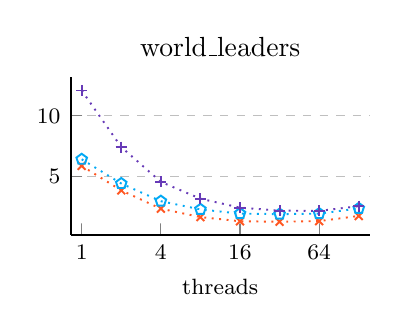
\begin{tikzpicture}
\begin{axis}[
  title={world\_leaders},
  xlabel={threads},
  xmode=log,
  log basis x={2},
  %ymode=log,
  log ticks with fixed point,
  plotParallel,
]
%% MULTIPLOT(algorithm|ptitle|attr)
%% SELECT threads AS x, AVG(lz_and_z_time/1000.0) AS y, "par \LPF" as ptitle, "parLZ" AS attr, MULTIPLOT
%% FROM parallel_stats
%% JOIN algorithm_meta_data ON algorithm = algorithm_name
%% WHERE input LIKE '%world_leaders%' AND tau=4 AND max_leaf_size=16
%% GROUP BY MULTIPLOT,x ORDER BY sorting_order
\addplot[parLZ] coordinates { (1,5.85533) (2,3.82267) (4,2.30467) (8,1.611) (16,1.26367) (32,1.22467) (64,1.27767) (128,1.70467) };
\addlegendentry{par \LPF};
  
%% MULTIPLOT(algorithm|ptitle|attr)
%% SELECT threads AS x, AVG(construction_time_ms/1000.0) AS y, "par BT w/o RS" as ptitle, "parWoRS" AS attr, MULTIPLOT
%% FROM parallel_stats
%% JOIN algorithm_meta_data ON algorithm = algorithm_name
%% WHERE input LIKE '%world_leaders%' AND tau=4 AND max_leaf_size=16
%% GROUP BY MULTIPLOT,x ORDER BY sorting_order
\addplot[parWoRS] coordinates { (1,6.40167) (2,4.39033) (4,2.92767) (8,2.24633) (16,1.89867) (32,1.854) (64,1.89567) (128,2.33033) };
\addlegendentry{par BT w/o RS};

  
%% MULTIPLOT(algorithm|ptitle|attr|attr)
%% SELECT threads AS x, AVG(construction_time_with_rs_ms/1000.0) AS y, "par BT with RS" as ptitle, "parRS" AS attr, MULTIPLOT
%% FROM parallel_stats
%% JOIN algorithm_meta_data ON algorithm = algorithm_name
%% WHERE input LIKE '%world_leaders%' AND tau=4 AND max_leaf_size=16
%% GROUP BY MULTIPLOT,x ORDER BY sorting_order
\addplot[parRS] coordinates { (1,12.1043) (2,7.41533) (4,4.53) (8,3.13433) (16,2.39333) (32,2.14367) (64,2.125) (128,2.51233) };
\addlegendentry{par BT with RS};

\legend{};

\end{axis}
\end{tikzpicture}
\end{tabular}

\end{document}
